\subsection{Radiation Monitoring System Design}
\label{sec:Radiation Design}
\subsubsection{TimePIX Control System}
The Raspberry Pi has proven to operate at float altitudes both from the previous SORA flight and other HASP payloads from previous years and as such was chosen again to host the control and analysis software. Both TimePIX devices were interfaced with the RPI via USB and controlled via the pypixet library developed at CERN by (Daniel Turcek?). The control software was designed to allow the configuration of the detectors via serial command and the downlink of device temperature, dose from ionizing radiation, and device counts. 
\subsubsection{Software Design}
Because the pypixet software blocks when exposing the detector for collection, both detectors had to operate in their own threads to allow the main thread to process uplink commands and control other systems. Data from each of these threads was then placed onto a queue where the main thread could periodically check if there was data ready to be processed. When a frame from one of the detectors was ready to be processed the main thread performed the analysis and then downlinked the results. Consequently, downlink speed was directly tied to shutter speed. An overview of the software design is shown in Figure \ref{softwaredesign}.
\begin{figure}[h!]
	\begin{center}
	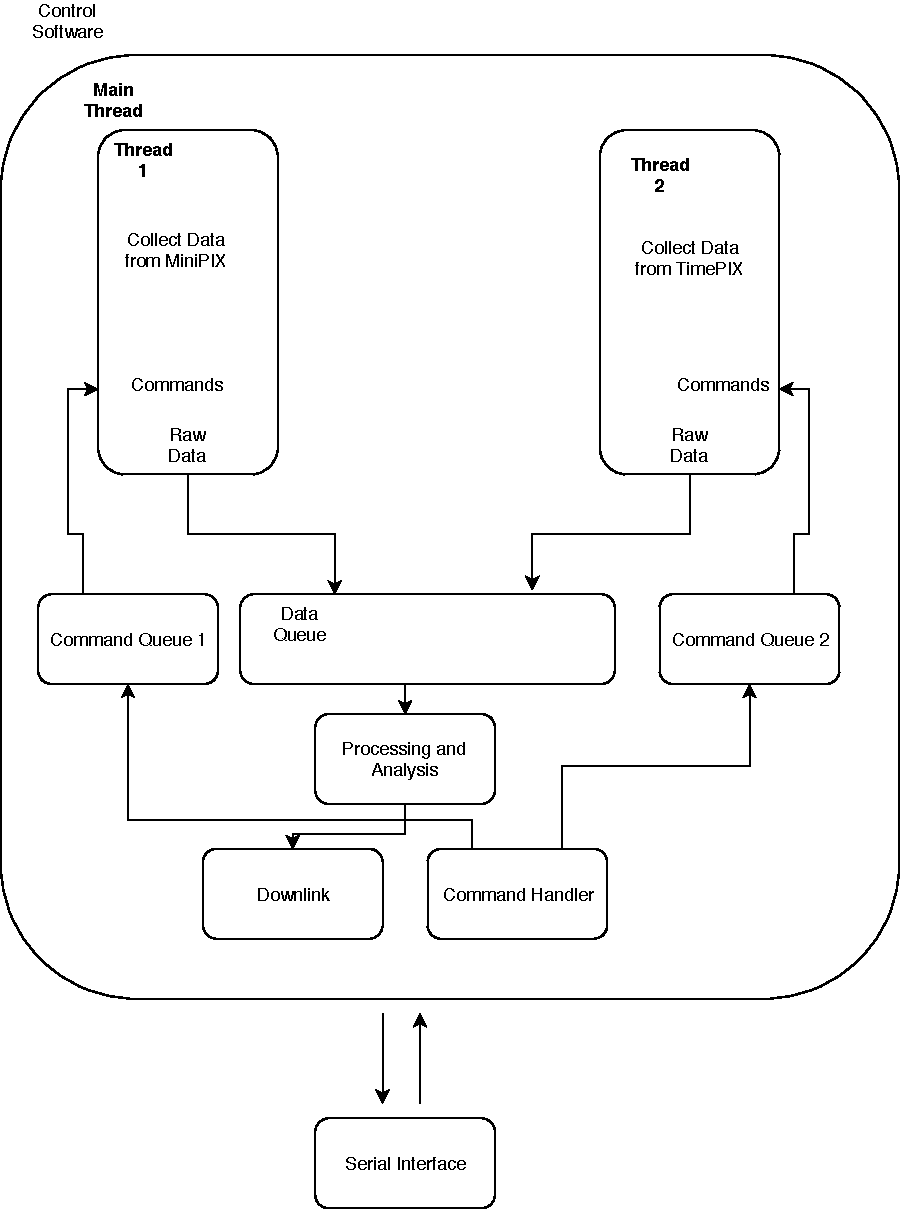
\includegraphics[width=0.6\textwidth]{figures/SoftwareDesign.pdf}
	\caption{Software design for the radiation control systems.}
	\label{softwaredesign}
	\end{center}
\end{figure}
\subsubsection{Thermal Considerations}
\subsubsection{Integration Testing}
\begin{figure}[h!]
	\begin{center}
	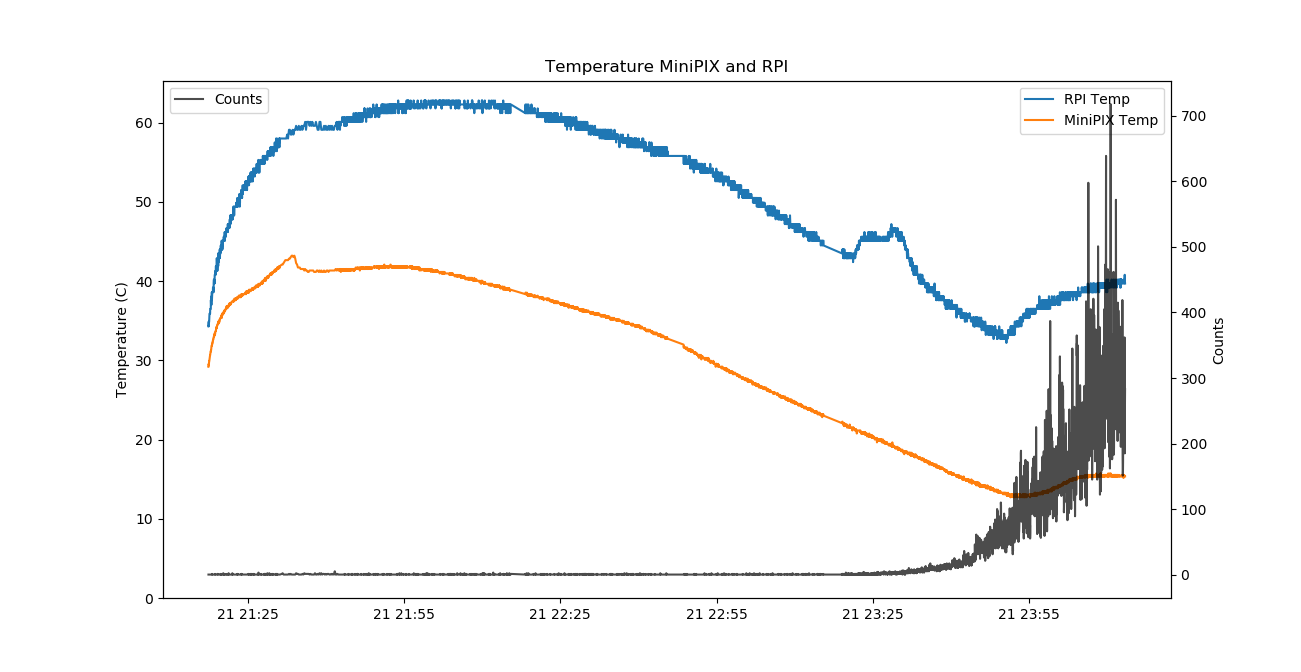
\includegraphics[width=\textwidth]{figures/tempsandcountsvtime.png}
	\caption{Temperature of flight computer and detector and counts.}
	\label{fig:integrationtemps}
	\end{center}
\end{figure}
